

guj2 <-- guj1



\section{Target Description}

Northern Gujarat is a marginal environment between the Thar Desert and the more fertile area of
Saurashtra. This region is an ecotone, characterized by the seasonal influence of the monsoon where
contrasting ecological niches are in tension and small climatic shifts can generate significant
environmental changes, eventually affecting resource availability. Archaeological evidence points to
the presence and possible coexistence in the area of groups of people with different resource
management strategies and mobility behaviors: hunter-gatherers (HG); agropastoralists (AP).
The aim of this study is to model resource management and decision making among hunter-gatherer
groups in this region to explore adaptive trajectories and performance in relation to a) environmental
variability and b) the appearance of other specialized groups.
What factors play a role in HG persistence or disappearance in arid margins? Is the advent of agro-
pastoral behaviour a big enough change to explain the disappearance of HG behaviour? Does climate
variability affect HG behaviour?
The model description follows the ODD (Overview, Design concepts, Details) protocol for describing
individual- and agent-based models (Grimm et al. 2006, 2010).

The agent-based simulation here proposed explores the potential for the persistence of hunter-gatherer
(HG) communities relative to climate-driven environmental change during the Holocene in N Gujarat, a
semi-arid region in NW India.
The model description follows the ODD (Overview, Design concepts, Details) protocol for describing
individual- and agent-based models (Grimm et al. 2006, 2010).


Note:
The modeling workflow is following these steps:
1. Environmental settings and climate engine
2. Resources and energy flow
3. Socio-ecological behaviour of HG
4. Socio-ecological behaviour of AP
5. Cultural transmission

This scaling approach includes three main theoretical and methodological research aspects:
1. Human behavioral ecological approach and socio-ecological co-evolutionary framework
2. Model based vs rule based action planner of the agents
Up to the date, steps 1, 2 and 3 have been developed . Work regarding AP models and cultural
transmission is in progress.



\section{Purpose}
In our starting hypothesis HG groups are adapted to marked seasonality (represented by the
monsoon) in the arid margins of northern Gujarat. We intend to explore HG resilience (Holling 1973,
Carpenter et al. 2001) considering climate variability.

Future : We intend to explore HG resilience considering the appearance of AP

\section{Entities, state variables, scales}


The model is designed to explore separately socio-ecological behaviours of two isolated populations: 1)
Hunter-Gatherers (HG) agents and 2) Agro-Pastoralist (AP) agents. This separate simulation of the
two groups is needed to obtain independent, coherent and consistent models of HG and AP decision
making. Once the dynamics of the modeled systems are understood for each population, agents from
the two populations will be combined in a single simulation execution. These will be considered as
independent groups, and interaction between agents will be limited to other agents belonging to the
same population. But the scope of this work is focused on exploring the socio-ecological behaviour of HG populations.

Agents from one population will interact within a given territory. It is characterised in terms of: a)
geographical information derived (height, slope), and b) landscape (soil types, resources). This
territory and its characteristics will generate an environment that will allow to portray differences in
strategies regarding settlement, mobility and resource use.


\subsection{Scales}
\paragraph{Agent Scale}
The basic agent is defined as a couple (one woman and one man). This is considered to be the entity
engaging in all decision-making processes and actions modeled in the simulation.
\paragraph{Time Scale}
Time Scale for the simulation is one day. This time step is coherent with the granularity of agents’
planning. The decision making of HG happens at the level of their daily action.
%%TODO recorda el pas que es va fer de SEASON a DAY... posar la rao perque es va fer 

\paragraph{Space Scale}

The spatial resolution of the proposed simulation model is constrained by the resolution of available
relevant geographic data and the nature of the agent mobility and resource gathering activities being
modeled.
Hence, it was decided to use 31.5m x 31.5m cells, corresponding to ca. 1000 square meters. This is
the level of resolution of the most detailed geographical information available for the area. This surface
fits the type of settlements recognized from archaeological surveys.


\subsection{Environment}
The simulation environment is large enough to develop all potential processes defined by the model according to the
experts' advice. It extends over an area of 50 Km x 50 Km (2500 Km2). Space is represented as a regularly spaced grid
of cells (a raster map). Each cell is a square of 31.5 m per side, and the total size of this environment
translates into a space of 1600 x 1600 cells (50,400 m x 50,400 m).
The ground model includes elevation and land features. Elevation is determined by a Digital Elevation
Model (DEM), a raster map containing the elevation value for each cell calculated from contemporary
satellite imagery. Land characteristics are reduced to three elemental categories:

\begin{enumerate}
\item Water: represents rivers and lakes.
\item Dune: represents the top area of the dune, which can be settled. Home location of the
agent will always be in a dune cell.
\item Interdune: represents the interdune(between water and dune) area where resources grow. The different land
features do not seasonally change in extension but their productivity (in terms of moist content
and therefore resources supported) does.
\end{enumerate}

The cornerstone of our environmental modeling is the climatic 'engine'. The climate module
determines the quantity of rain that precipitates evenly on the landscape on every time step.
Precipitation is used in conjunction with the terrain model to calculate the amount of biomass for each
cell and season. The climate model is based on historical data, as well as Holocene monsoon models.


\subsubsection{Climate}

The focus on resource utilization strategies within a particular environment requires to make explicit
the potential variations in the landscape. In particular for our case study, the presence of the monsoon
generates a strong seasonality (asymmetrical precipitation patterns).
Monsoon seasonality determines the presence of three critical “moments” in simulation time, each
spanning 4 months. Therefore, the seasonal subdivision in three periods will be repeated in a cyclical
way as follows below. Identification of months from western calendar covered by each of the seasons is done 
taking the first letter of the month name and using the concatenation to label the season. So "JJAS" stands 
for the season that covers June, July, August and September, for instance. "ONDJ" is the label for the 
season covering October, November, December, January. "FMAM" is for February March April May.    


\begin{enumerate}
\item JJAS (rain season: high precipitation, high temperature, low evapotranspiration)
\item ONDJ (post-Monsoon: low precipitation, cool temperature, medium evapotranspiration)
\item FMAM (dry season: low precipitation, high temperature, high evapotranspiration)
\end{enumerate}


It is important to note that any given “year” in the model starts with the beginning of the rain season
(June). In fact, virtually all rain in the region is carried by the monsoon that falls between June and
September (JJAS). Therefore, it is during the JJAS season that the totality of the generated yearly
precipitation value is calculated (following a Gamma distribution). No additional precipitation is
considered for the remaining eight months of the year (ONDJ and FMAM).

\subsubsection{Resources}

Each cell has a finite number of resources. Resource availability for each cell is calculated from the
following variables:

\begin{enumerate}
\item Yearly precipitation (rainfall, using a Gamma distribution)
\item Type of cell (Water Body, Interdune, Dune)
\item Mean yearly Biomass per cell and type.
\item Cell history (e.g. whether the cell was used for crop in a previous step or part of the resources
were consumed before).
\end{enumerate}

Resources include the total biomass that can be found in a cell (fauna and flora). They are exploited
by HG agents engaging into foraging activities. Foraging includes activities such as hunting animals
and gathering plants, fruits, seeds, etc. Indeed, from a literature review it is clear that secondary
biomass production (animals) is directly related to primary biomass quantity. Moreover, as there is no
interest in our simulation to explore gender-based labour division we decided to consider hunting and
gathering as a single activity (foraging) without distinguishing between plant or animal utilization. In the
light of this, it was decided to consider a value for cell (dune vs interdune) based on published
information of primary biomass production in desert (dune) and savannah (interdune) biomes (after
Kelly 1983 – Table 3).


\begin{table}[ht!]
\centering	
	\begin{tabular}[c]{|l|l|l|l|l|}
	\hline
	Cell Type & Yearly Primary Biomass Production & Efficiency & Energy & KCal \\
	\hline
	Dune (desert) & $700g/m^2$ & $13\%$ & $1820KJ/m^2$ & $435KCal$ \\ 
	\hline
	Interdune (savanna) & $4000g/m^2$ & $23\%$ & $18400KJ/m^2$ & $4395KCal$ \\
	\hline
	\end{tabular}
	\caption{Parameters for resource parametrisation according to Kelly (1983; Table 3, p. 284).}
	\label{tab:tabResources}
\end{table}

\begin{enumerate}
 \item Cell area = 1000m2
 \item 1 g Primary Biomass = 20KJ
 \item 1 kcal = 4.184 KJ
\end{enumerate}



\paragraph{Distance to water}
This average value of resources is modified based on the distance of a cell from the closest
water body. This weight decreases linearly to the distance, and models the heterogeneity of
biomass generated by a higher presence of flora and fauna near the zones where needed
water can be collected. The update due to resource growing will depend on the matrix of distances
to the nearest water body representing this information.

\paragraph{Efficiency}
The total primary biomass value does not constitute the entire primary biomass available for
consumption to animals and humans. This value represents the entire biomass production
including both edible (fruits, tubers some roots etc.) and non-edible (wood, stems, branches
etc.) parts of the plants. The ratio of profitable biomass versus whole biomass will be the
efficiency value specified in the above table that allow to calculate the energy effectively
available for humans.

\paragraph{Domesticated cell} (work in progress)
The model is prepared to tag cells wether they are domesticated or wild when we will introduce AP 
agents in the runs\pdfcomment{ho deixo aqui o a future work?}. Domesticated plant resources define the density of domesticated plants found inside the cell. It is important to note that wild and domesticated types of resources 
are mutually exclusive: i.e. wild resources are not found on cultivated plots. 

The basic idea for a domestication cell is that of small scale shifting cultivation, in which a plot is
cultivated following a cycle that includes abandonment so to allow soil properties to recover. A
domesticated cell can be planted for a maximum of three consecutive years. It then needs to be
abandoned for a minimum of three years (during which it will be considered as Fallow). After three
years of abandonment the cell becomes wild and can be used again for agriculture. If a plot is
abandoned before being cultivated for three consecutive years it will have to remain abandoned for
the same amount of years it was worked. During these years it will remain fallow, after that it will
become wild again.

Crop cells change temporary their state to Fallow during the FMAM season, where no agricultural
uses can be executed. It turns to Crop again during JJAS season, and will be ready to sow at the end
of it.


\subsection{Agents}
The following attributes have been chosen to account in our model.

\begin{enumerate}
\item[Age] - A numeric variable that keeps track of how many time steps a given agent has been
active in the simulation.
\item[Children] - A collection of human entities. The number of children is bound by resource
availability. Birth and mortality rates depend on resource availability and hence regulate the 
number of children.
\item[Home location] - the cell where the agent resides and the spatial centre of the activities it
carries out. Any number of agents can share a given cell.
\item[Home range] - Maximum distance an agent may travel in one day. This attribute restricts
foraging and social activities from taking place in cells too far from the agent Home location.
The area enclosed in the circle of radius “Home range” is divided in six equal sectors. Such
division models the idea of direction of exploration for the agent actions, while simplifying the
decision-making process (an agent will choose to forage in one of the six sectors,
independently of single cells).
\item[Food needs] - Value that sets the minimum calories a given individual needs in each time step
in order to survive. The total amount of food needs for an agent is computed as the sum of the
food needs of the individuals that form a given agent. The probability of death increases for all
the individuals that form a given agent when this basic quantity of resources is not foraged
within a day (due to starvation). Needs are defined by the following table:
\iem[Available forage] - Daily time that an agent can spend on foraging. The total amount of
foraging time for any given agent is computed as the sum of the foraging time of the
individuals that compose it. Foraging time increases from infancy to adult life, modelling
learning processes as defined in the following table:


\end{enumerate}

%%TODO FUTURE

%\item Relationships – These are the connections between agents. The following types of
%relationship are considered:\\
%	\begin{enumerate}
 
%	\item Acquaintance – This is the result of having met at some time in the past. A numeric
%	value is used to track the intensity of the relationship. This value changes with and
%	depends on the actions of the involved agents.\\
%	\item Next Of Kin – Agents connected by family ties (the agents have some common
%	ancestor). The closeness of the family tie is also modelled with an intensity value that
%	remains constant throughout the agent's life. The value is inversely proportional to the
%	distance in the genealogical tree.

%	\end{enumerate}



\begin{figure}[h]
\centering
\setlength\fboxsep{0pt}
\setlength\fboxrule{0.5pt}
\fbox{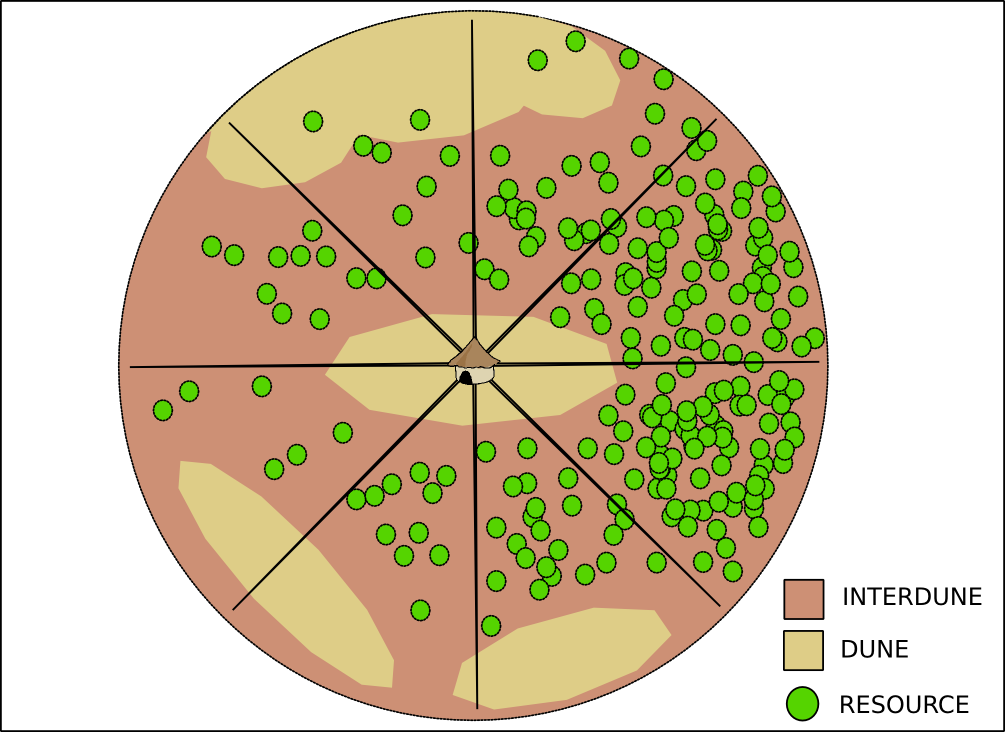
\includegraphics[width=60mm,keepaspectratio=true]{figures/sectors.jpg}}
\caption{Figure. Home range division for foraging and moving home actions}
\label{fig:sectorsDivision}
\end{figure}


Tables. Individual caloric requirements (left), Individual foraging time (right)

figures pg35 


\section{Process overview and scheduling}

Execution follows two time-scales. On the one hand, three processes (‘yearly precipitation’, ‘biomass
yearly production’ and ‘population size adjustment’) are executed once every year. On the other hand,
agents decision-making processes are updated on a daily base. The simulation follows this schedule,
beginning the first day of the JJAS season:
For each year:
\begin{enumerate}
	\item 1. Precipitation calculation
	\item 2. Biomass yearly production
	\item 3. For each day of the year:
	\begin{enumerate}
		\item a. Daily biomass availability
		\item b. Agent planning:
		\begin{enumerate}
			\item i. Knowledge update
			\item ii. Choice of actions
		\end{enumerate}
		\item c. Execution of agents actions
	\end{enumerate}
	\item 4. Population size adjustment
\end{enumerate}


Details for each simulation phase are given hereafter.


\subsection{Precipitation calculation}
The total amount of rain is calculated as a random number following the Gamma distribution defined in
section 7 (Input Data)
\subsection{Biomass Yearly Production}
The biomass that a cell will produce in an entire year is calculated from rainfall and mean year
production for its particular type, provided by historical records.
We consider a linear relation between rain and biomass production. The deviation of rain in a given
year from the period mean allows interpolating the amount of biomass deviation from the yearly mean
biomass. That is, if the mean of rain is 100 liters and the climate model produces 80 liters the deviation
to apply is 20\%, and for that year the biomass will be a 80\% of the mean yearly production for the
period.

\subsection{Daily processes}

\subsubsection{Biomass availability}
Yearly biomass production does not appear immediately in the cell in the first day of JJAS season.
Resources increase gradually, following a cumulative pattern that accounts for the progressive
accumulation of water through JJAS, until the beginning of ONDJ. From then on, resources decrease
linearly to the end of the year, then, they reach a percentage of the highest peak defined by the ‘end-
of-year minimum residual resources’ parameter (EMR). Variations in EMR does not affect overall
yearly biomass production so that the higher the EMR, the lower the maximum peak of resources at
the JJAS-ONDJ boundary.


\begin{figure}[h]
\centering
\setlength\fboxsep{0pt}
\setlength\fboxrule{0.5pt}
\fbox{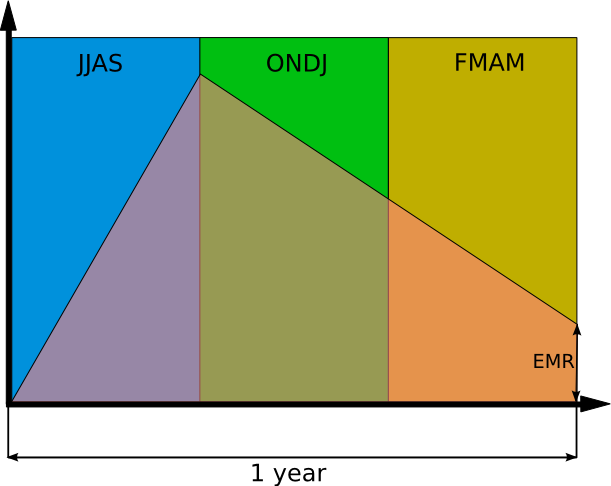
\includegraphics[width=120mm,keepaspectratio=true]{figures/resGrow.png}}
\caption{Figure. Modelled biomass availability through the year.}
\label{fig:resourceGrowing}
\end{figure}


\subsubsection{Agent planning}
Each day the agent will update its knowledge about environment and choose an action to execute (the
decision-making process is defined in the Submodels section 8). The list of available actions is:
\begin{enumerate}
\item Forage - The agent takes multiple walks of a bounded length computed from available
foraging time. Walks are limited to the agent’s Home range. From the visited cells, resource
reward is retrieved based on biomass of the cells. The agent will halt the walk when reward
achieves food needs.
\item Move home - The agent moves from its current home location to a new one within Home
range. The new home settlement is chosen randomly between the dune cells situated in the
richest sectors (containing the highest amount of resources) within Home range. Afterwards, a
Forage Action is executed using half the available daily Foraging time of the agent in order to
include the time spent on movement.
\end{enumerate}


\subsubsection{Adjustment of agent population size}
This processes are executed for each agent:

\begin{enumerate}[1-]
	\item Age. Agent aging (increment human objects age).
	\item Death. Every individual inside an agent will have a probability of dying. At the end of the year
	every individual within an agent must pass two tests to survive:
	\begin{enumerate}
		\item Natural death. Every individual has a 1.5\% annual death probability, except during the
		first four years of life, when this probability is 10\%.
		\item Starvation. Depends on the capability of an agent to fulfil its caloric requirements. Every
		day the agent computes the percentage of needed resources that it was unable to collect.
		This 'starvation value' is accumulated through the year. The cumulative starvation value is
		translated into the overall percentage of full days of the year in which the agent was
		unable to gather sufficient resources. This percentage is translated at the end of the year
		as the probability for the agent to die of starvation.
	\end{enumerate}
	\item Removal. If all the individuals that form an agent are dead, the agent will be removed from
	simulation.
	\item Reproduction. At the end of the year every agent where both adults are still alive will have a
	50\% chance of having a new child.
	\item Emancipation. An agent with individuals coming of age will seek suitable matches among
	agents within its social range. When two individuals coming of age from different agents join a
	new agent is created.
\end{enumerate}

\section{Design concepts}

\subsection{Basic principles}
The behavior defined in this model is derived from the Optimal Foraging Theory (OFT)\ref{blabla}, developed
within behavioral ecology and Rational Choice Theory(RCT)\ref{blabla} from economics. The main principle of OFT is the maximization of long-term energy gain. In other words, it is usually assumed that animals attempt to maximize the benefit to cost ratio. Evidence exists e.g. among great tits(Parus major), birds that show relatively successful strategies in terms of OFT. Although it is doubtful whether humans attain the optimal rate of energy gain, they do succeed in improving their
foraging efficiencies, or 'memorising'. Also, RCT framework backs the decissions of not taking a choice that implies
some negative outcome. The term Rational stands for balancing cost of choices in a way that maximizes personal advantage.



\subsection{Emergence}
The model explores the emergence of stable HG populations under different climatic conditions.
%%TODO 
%% afegir la part de comparació amb hard-wired technique vs UCT --> adaptació (BSC day)

\subsection{Adaptation}
At the present moment the model is not interested on the emergence of individual adaptive traits, and
for this reason adaptive options for the agents are limited to the decision making process. The different
agents try to respond to the dynamics of environment choosing Home locations and Foraging actions
depending on their particular situation. The aim is not policy discovering, just adaptative planning.
Adaptive options for the agents are based on the complexity of the decision making process. Actions
costs and outcomes are predefined following the model's configuration, but the order and the use of
them is entirely an agent's choice. Following this reasoning, the different agents will try to adapt the
dynamics of environment (both ecological and social) planning a different set of orders each time step.
\pdfcomment{ATM:future work}A further step in this model will see agents with mixed pool skills that are capable of choosing actions typical of HG and AP populations. Each agent will have different efficiency values for different actions, that will vary in time. In this way, the agent will also adapt specializing its actions.


\subsection{Objectives}
Following the basic principles stated before, the objective for any agent is the survival of its individuals.
This assumption is clearly from optimizing the system, as the different populations won't be guided by
the mission of 'colonizing' the entire landscape. Anyway, this outcome will be seen following
evolutionary mechanisms and positive selection. Well adapted agents will have more possibilities to
survive, thus creating more children and agents with similar cultural traits.

\subsection{Learning}
Foraging learning process is modeled using vertical transmission. A child gradually learns to forage in
an efficient way, and for this reason the available foraging time contributed by children increases until
adulthood.
\subsection{Prediction}
An agent does not keep track of previous rainfall values, so it is not able to predict the future state of
the environment.
\subsection{Sensing \& Information Retrieval from Environment}
An issue seldom addressed in the literature of ABM applications into Social Sciences is the fact that
agents do not have perfect information on their environment. Home range limits the zone that agent
know around its home location. Other issues about bounded rationality is treated in the smart agent section.
 
\subsection{Interaction}
The interaction between agents is currently limited to the \emph{fission} process that is executed when two
agents with adult children are inside social range, and to \emph{information sharing} at the end of the day.


\subsection{Stochasticity}
Stochasticity is used in three different concepts:
\begin{enumerate}
\item Environment. Precipitation is calculated as a estochastical process following a Weibull
distribution.
\item Outcomes. Some actions have different outcomes depending on stochastic processes,
like forage and harvest. It encapsulates the complex process of resources collection (i.e.
risk, variability, etc.), and it is important due to the fact that Actions will be chosen
depending on their outcomes and risk of failure.
\item Life events. Death and reproduction are stochastic processes following realistic
distributions.
\end{enumerate}

\subsection{Collectives}
The agent, atom of the decision-making process, is itself a collective of different related individuals.
\subsection{Observation}
Population dynamics are the most important concepts to derive from the model.

\section{Initialization}
Initial state of the model is divided by entities:

6.1 Climate
Rainfall yearly precipitation is a stochastic value calculated from input data, as seen in section 7\pdfcomment{dynamic link}.
Calculated values depend on the initialization seed used in the random number generation, that is
stored as a parameter of the model's configuration. Next parameters can be modified during
initialization time:
	\begin{enumerate}
	\item[EMR] End-of-year minimum residual resources
	\item[AYP] Average Yearly Precipitation
	\item[VYP] Variance in yearly precipitation
	\end{enumerate}


\subsection{Environment}
Ground Model and land features are raster maps created from real data (see also section 7\pdfcomment{symbolic link}). The
model is able to load any raster map with correct values. This process is done during init time from the
file specified in the configuration.


\subsection{Resources}
The conversion functions that create available biomass from landscape and rainfall for each cell use
parameters specified in the configuration. They are based on published research; nevertheless they
can be modified in order to explore different plausible scenarios.

\subsection{Agents}
Several parameters can be changed from the configuration. These values are loaded during init time,
and remain stable during the entire execution. This is the list of parameters used for this model:

\begin{enumerate}
	\item Life-event related:
	\begin{enumerate}
		\item Adulthood age: 15
		\item Dying age (HG/AP): Stochastic distribution %%TODO put a number
		\item Number of agents 
	\end{enumerate}
	\item Resource related:
	\begin{enumerate}
		\item Home Range: 300 cells
		\item Number of sectors: 8
		\item Forage time cost: 30 minutes
		\item Walking Speed: 3 km/hour
	\end{enumerate}
\end{enumerate}


\section{Input data}

\subsection{Rainfall}

Rainfall (yearly precipitation) is the 'environmental engine' of the model. Data for precipitation rate are
extracted from historical data (1871 - 2008). The climate engine is defined as a probability distribution,
from which the total precipitation during a year is derived. The Gamma distribution was the best fit for
the available rainfall dataset.

pg38 gamma fitting graphic
Gamma distribution and historical data
Figure. Precipitation Gamma distribution

codi R del fitting

first approach : weibull --> could not play with mean,stdev values : complex functions for conversion
of mean-stdev to alfa-beta
gamma : same shape, high fitting, (it is pending to calculate a goodness measure) -> easy conversion to and
from mean-stdev

//* posa el codi en R per extreure el parametres GAMMA
/*
primer varem usar una weibull perque trobavem millor fit.
voliem jugar amb la mean i la stdev. Implicava calcular funcions gamma per alterar
l'alfa i la beta de la weibull. Calia resoldre certes integrals. I vam veure mes senzill
modelar amb una gamma. Shape encaixa quasi tant be i podem treballar directament
amb mean/stdev. La transformacio a alfa/beta de la gamma es quasi directe.
*/


%%TODO end gamma part  


\subsection{Ground Model}
This model is derived from LANDSAT and ASTER satellite imagery (combining pre- and post-monsoon
imagery) and includes DEM and land features. Satellite data are transformed using unsupervised
classification and clustered in the 3 classes (water, interdune and dune). The model is exported as a
Raster map.

\pdfcomment{ATM:future: passarem de 3 categories a 5 de terra. tindrem mes water bodies, rius, etc}


\subsection{Hunter-Gatherer behavior}
Archaeological data are incomplete and limited in terms of derivable behavioural patterns. HG
behaviour for the model was derived from published studies of historical and present-day populations
in similar ecological settings. There are groups of HG that live near N Gujarat (the Van Vargis, see
Nagar 2008). However, these communities have a high degree of interaction with and dependency
from settled agricultural communities for their subsistence strategies. This occurrence constitutes a
strong bias towards the use of these groups to model our HG agents. Instead, we used as surrogates
of our HG population, African groups of the San communities.
Among living and historical HG communities, the San (especially the G/wi and G//ana groups of
Botswana) represent the best-fitting parallel in terms of ecosystem (Tanaka and Sugawara 1996).
These groups are found on a flat plateau in the central part of the Kalahari desert. The landscape
morphology is characterised by fossil rivers and traces of sand dunes. Rainfall is concentrated in the
summer months with c. 400 mm annual average precipitation. The vegetation of the area is dominated
by plants of the Gramineae family (grasses) and a mixture of shrubs of the same genus/families that
are found in North Gujarat.

\pdfcomment{AMT:pg39 : poso la taula de surrogates??? nomes esmentar-los?}

\section{Submodels}

\subsection{Agent execution cycle}
The majority of Agent-Based Models mix knowledge acquisition, decision-making and execution in the
same phase of an agent's execution. This choice is useful if we deal with agents with simple decision-
making processes where the choice of behaviors is predefined. However, this classical approach to
ABM has a major drawback, and is the fact that the agent will have scripted strategies, and for this
reason it won't be able to choose strategies different from the ones defined there.
The model proposed here splits the different phases. During each time step every agent updates its
knowledge about the environment (possibly including other agents). This action is combined with a set
of possible actions, in order to choose which plan of actions will be executed. Several factors can be
used to enrich the process:

%%TODO no acabo de pillar tot aquest paragraph. es aixi?


\begin{enumerate}
	\item Agent's goals and agent's preferences referred to the choice of particular actions
	\item The information that the agent perceives from the environment and the reliability of such
	information.
	\item The information collected from other Agents, as well as its reliability.
	\item The feedback the agent receives from engaging into a given activity.
	In this particular model the goal of every agent is to maintain alive its individuals, and the potential
	actions are the ones defined in the document.



 This approach will allow to integrate Artificial
	Intelligence techniques into the current decision-making process, depending on particular research
	around this first model.

\end{enumerate}


The execution of the agents during each time step is divided in three different phases:
\begin{enumerate}[1.]
	\item[Knowledge update]
	The agent collects information from the environment, and creates an individual representation of the
	world using its preferences and objectives. Agents will calculate the amount of biomass available in
	each directional sector (utility score), as well as potential settlement zones.
	\item[Action choice]
	The agent decides which actions to execute once knowledge has been collected, based on the
	following steps:
	\begin{enumerate}
		\item Agents checks whether there is any sector inside its home range where resources can be
		obtained. This is calculated based on available foraging time and resources on cells.
		\item If needed resources can be obtained the agent will choose to Forage in one of the Sectors
		where this is possible.
		\item If this is not possible, the agent will choose to Move Home. A collection of possible new homes
		is created based on the quantity of resources inside the Home range from this new location.
		The final location is chosen amongst the ones that fulfill resource requirements.
	\end{enumerate}
	\item[Action]
	After every agent has defined a plan, all of them are executed sequentially following a randomized
	order.
	\item[Information Sharing] 
	Once actions of the day are executed the pipeline proceeds with the information
	sharing phase.
\end{enumerate}


9
References

Carpenter, Steve, Brian Walker, J. Marty Anderies, and Nick Abel (2001). “From Metaphor to Measurement:
Resilience of What to What?” Ecosystems 4: 765–78 1
Grimm V, Berger U, Bastiansen F, Eliassen S, Ginot V, Giske J, Goss-Custard J, Grand T, Heinz S K, Huse G, Huth A,
Jepsen J U, Jørgensen C, Mooij W M, Müller B, Pe’er G, Piou C, Railsback S F, Robbins A M, Robbins M M,
Rossmanith E, Rüger N, Strand E, Souissi S, Stillman R A, Vabø R, Visser U and DeAngelis D L (2006). “A standard
protocol for describing individual-based and agent-based models”. Ecological Modelling 198 (1-2), 115-126.
Grimm V, Berger U, DeAngelis D L, Polhill J G, Giske J and Railsback S F (2010). “The ODD protocol: A review and
first update”. Ecological Modelling 221 (23), 2760-2768.
Holling CS (1973). “Resilience and Stability of Ecological Systems Annual Review of Ecology and Systematics Vol. 4:
1-23.
Kelly, R.L. (1983). Huter-gatherer mobility strategies. Journal of Anthropological Research, 39(3), 277-306.
Nagar, M. 2008. Hunter-gatherers of North and Central India: an Ethnoarchaeological Study. BAR International Series
1749. Arcaheopress: Oxford.
Tanaka, J., Sugawara, K. (1996). The /Gui and //Gana of Botswana. In In: Lee, R.B. And Daly, R. (eds). The
Cambridge Encyclopedia of Hunters and Gatherers, CUP, Cambridge, pp. 195-199.












